
%
% verslag.tex   30.11.2017
% Voorbeeld LaTeX-file voor verslagen bij Kunstmatige Intelligentie
% http://www.liacs.leidenuniv.nl/~kosterswa/AI/verslag.tex
%
% Gebruik:
%   pdflatex verslag.tex
%

\documentclass[10pt]{article}

\parindent=0pt

\usepackage{fullpage}

\frenchspacing

\usepackage{microtype}
\usepackage[a4paper, total={6in, 9.5in}]{geometry}
\usepackage[english,dutch]{babel}
\usepackage{multirow}
\usepackage{changepage}
\usepackage{graphicx}
\usepackage{amsmath}
\usepackage{listings}
% Er zijn talloze parameters ...
\lstset{language=C++, showstringspaces=false, basicstyle=\small,
  numbers=left, numberstyle=\tiny, numberfirstline=false, breaklines=true,
  stepnumber=1, tabsize=4, 
  commentstyle=\ttfamily, identifierstyle=\ttfamily,
  stringstyle=\itshape}

\usepackage[setpagesize=false,colorlinks=true,linkcolor=red,urlcolor=blue,pdftitle={Het grote probleem},pdfauthor={Sebastiaan Alvarez Rodriguez & Andrew Huang}]{hyperref}

\author{Sebastiaan Alvarez Rodriguez (s1810979) \and Andrew Huang (s1913999)}
\title{
    Neurale netwerken \\
        \large Een lerende computer
}


\begin{document}

\selectlanguage{dutch}

\maketitle
\begin{figure}[h]
	\begin{center}
		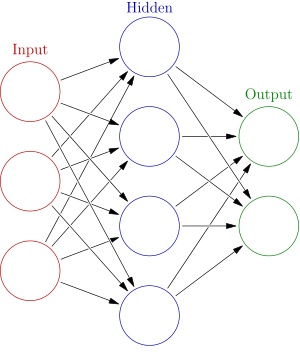
\includegraphics[]{images/nn.png}
		\caption{Een neuraal netwerk \cite{image}}
	\end{center}
\end{figure}

\clearpage

\section{Inleiding}
Dit is de vierde practicumopdracht van het vak AI: Neurale netwerken. Deze opdracht is \href{http://liacs.leidenuniv.nl/~kosterswa/AI/nn18.html}{\underline{hier}} \cite{assignment} te vinden.
Het doel van deze opdracht is om een neuraal netwerk te implementeren die het correcte antwoord van verschillende operaties, zoals XOR, OR en AND, kan geven.

\section{Uitleg probleem}
Het programma moet het correcte antwoord geven op de verschillende operaties. Het programma weet echter niet wat deze operaties doen; het weet niet eens wat een operatie is. Hoe een neuraal netwerk dit dan toch voor elkaar krijgt wordt verderop besproken. Het programma heeft een aantal argumenten die bepalen hoe goed het de verschillende operaties leert:

\begin{itemize}
    \item -a, de geaccepteerde foutmarge, deze marge bepaalt hoever een resultaat mag afwijken van het antwoord.
    \item -d, het aantal verborgen knopen, dit is het aantal knopen in de verborgen laag.
    \item -e, het aantal trainingssessies, dit is het aantal keren dat het programma "leert" wat het correcte antwoord is.
    \item -i, het aantal inputs, dit is het aantal inputs voor de verschillende operaties.
    \item -o, de operatie, dit is de operatie die moet worden geleerd door het neuraal netwerk.
    \item -r, het aantal keer dat de trainingssessies worden verlopen om het neurale netwerk te testen.
    \item -l, 1 als ReLU (wordt verderop besproken) wordt gebruikt anders wordt de sigmoid functie gebruikt.
\end{itemize}

\section{Relevant werk}
De informatie voor deze opdracht is te vinden op de \href{http://liacs.leidenuniv.nl/~kosterswa/AI/nn18.html}{\underline{website}} van het vak Kunstmatige Intelligentie \cite{assignment}. \\ \href{http://liacs.leidenuniv.nl/~kosterswa/AI/nnhelp.html}{\underline{Hier}} is te vinden de pseudocode voor het leerprocess van het neurale netwerk \cite{backprop}.

\section{Aanpak}
Het programma maakt gebruik van een neurale netwerk om het probleem op te lossen. Hoe dat precies te werk gaat wordt hier besproken.

\subsection{Het neurale netwerk}
Het neurale netwerk is ge\"inspireerd door het biologische neurale netwerk dat te werk gaat in de hersenen van organismen. Het bestaat uit lagen van knopen (neuronen), waarbij de eerste laag de invoer is van van het netwerk en de laatste laag het uiteindelijke antwoord bepaalt. Elke knoop in het netwerk krijgt alle inputs binnen van de vorige laag, wat een vector is, en doet een vermenigvuldiging met een matrix van gewichten. Figuur 2 \cite{chapter} beeldt dit uit. De uiteindelijke waarde van de knoop is deze vermenigvuldiging plus een bias waarde, gestopt in een activatie functie, wat een waarde teruggeeft tussen de 0 en 1 (in het geval dat de sigmoid functie wordt gebruikt). Op deze manier gaat de input door het neurale netwerk heen totdat het de laatste laag bereikt heeft, waarna een vermenigvuldiging leidt tot het antwoord van het netwerk. Het netwerk leert van het antwoord dat het produceert met behulp van Backpropagation. 

\begin{figure}[ht]
    \centering
    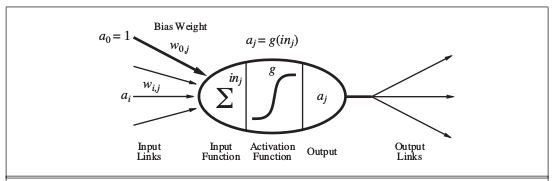
\includegraphics[scale=0.6]{images/neuron.png}
    \caption{Een neuron van het neurale netwerk}
    \label{fig:my_label}
\end{figure}

\subsection{Backpropagation}
Een neuraal netwerk stelt na elk verloop van het netwerk de gewichten en de bias bij om het gedrag van het netwerk te veranderen. Dit is hoe een neuraal netwerk progressief beter wordt in het vinden van het correcte antwoord. Hoe het netwerk dit doet is met behulp van een fout marge. Deze fout marge, $Err$ in ons netwerk is het verschil tussen het antwoord van het netwerk en het gewenste antwoord. Om de gewichten van de verborgen lagen bij te stellen, wordt eerst $Err$ en $\Delta$ uitgerekend. 

\begin{align*}
    Err & \leftarrow y - out \\
    \Delta & \leftarrow Err * g'(inout)
\end{align*}

Hier is y de gewenste output, out het antwoord van het netwerk, $g'()$ de gedifferenti\"eerde activatiefunctie en inout de input van de laatste knoop.
\\\\
Met behulp van deze $\Delta$, kan de $\Delta_j$ worden uitgerekend. Het idee van $\Delta_j$ is dat elke verborgen knoop $j$ een deel bijdraagt aan de fout $\Delta$ in elke output knoop waaraan het verbonden is. Dus de waarde van $\Delta_j$ op een willekeurige j is de "sterkte" van de verbinding tussen de knoop j en zijn outputknoop. Om concreter te zijn, hoe meer invloed een kleine verandering in j heeft op zijn outputknoop, hoe hoger de $\Delta_j$ waarde zal zijn. De $\Delta_j$ is berekend door:

\begin{align*}
    \Delta_j & \leftarrow g'(inhidden_j) \times W_j \times \Delta
\end{align*}
Waarin inhidden de input is van de j-de verborgen knoop en $W_j$ de gewicht van de j-de knoop naar de laatste laag.
\\\\
Nu de invloeden van elke knoop is berekend kan het daadwerkelijke terug propogeren beginnen.
De gewichten worden bijgesteld aan de hand van de $\Delta_j$, beginnend met de laatste laag:

\begin{align*}
    W_j \leftarrow W_j + \alpha \times acthidden_j \times \Delta
\end{align*}
Met $W_j$ de j-de gewicht voor output van de verborgen, $\alpha$ de constante leersnelheid van het netwerk en $acthidden_j$ de j-de output van de vorige verborgen knoop.
\\\\
En vervolgens de verborgen lagen:

\begin{align*}
    W_{i,j} & \leftarrow W_{i.j} + \alpha \times x_j \times \Delta_k
\end{align*}
Hier is $W_{i,j}$ de i -en j-de gewicht en $x_j$ de j-de input van het netwerk.
\\\\
Met dit algoritme wordt het netwerk na elke doorloop progressief beter in het vinden van een antwoord, doordat de gewichten steeds nauwkeuriger worden. Het netwerk stelt zijn gewichten bij, beginnend vanaf het einde van het netwerk terug naar het begin. Hierdoor wordt dit algoritme Backpropagation genoemd. De precieze berekeningen in het algoritme en verdere informatie is te vinden in hoofdstuk 18.7 van het boek "\textit{Artificial Intelligence: A Modern Approach}" \cite{chapter}.

\subsection{Activatie functies}
Het netwerk moet het antwoord op de operaties: XOR, OR en AND kunnen geven. Dit antwoord is 0 of 1. Omdat het netwerk geen binaire antwoorden geeft (anders zou het in 50\% het correcte antwoord geven), moet de output van elke knoop een getal zijn tussen 0 en 1. Om dit resultaat te krijgen wordt de output van elke knoop gestopt in een activatie functie. De meegeleverde functie is de sigmoid functie, die hogere waardes dichterbij de 1 brengt en lagere waardes dichterbij de 0. In de praktijk wordt voor diepere netwerken een andere functie gebruikt, de Rectified Linear Unit (ReLU). Dit is een functie in de vorm:

\begin{align*}
    f(x) & = max(0,x) \\
    f'(x) & =
            \begin{cases}
                0,& \text{if } x\leq 0\\
                1,& \text{otherwise}
            \end{cases}
\end{align*}

Het voordeel van ReLU is dat verborgen knopen uit kunnen worden gezet als ze teveel bijdragen aan een grote fout marge en dat de computatie veel sneller is dan bij andere activatie functies, zoals sigmoid \cite{relu}. In de experimenten verderop bekijken we de verschillen tussen de sigmoid en ReLU functies op het neurale netwerk.


\section{Implementatie}
Er is gekozen voor de programmeertaal C++. Verder is er een framework meegegeven die te vinden is \href{http://liacs.leidenuniv.nl/~kosterswa/AI/nn.html}{\underline{hier}}\cite{assignment}. Hierin is het neurale netwerk ge\"implementeerd.

\section{Experimenten}
Het programma dat het neurale netwerk draait heeft verschillende argumenten die de gebruiker meegeeft, zoals de leersnelheid, het aantal inputs, aantal knopen, aantal trainingssessies etc. In de volgende experimenten bekijken we voor elk van deze argumenten hoe verschillende hoeveelheden het netwerk be\"invloeden en wat een goede specificatie zou kunnen zijn voor ons neurale netwerk.
Elk experiment wordt gedaan met de volgende standaard specificaties, tenzij anders vermeld:

\begin{table}[ht]
    \centering
      $\begin{array}{ l | c | c}
        \text{Leersnelheid } \alpha & 0.1 \\ \hline
        \text{Geaccepteerde fout} & 0.1 \\  \hline
        \text{Aantal verborgen knopen} & 4 \\  \hline
        \text{Aantal trainingssessies} & 100000 \\  \hline
        \text{Aantal inputs} & 2 \\  \hline
        \text{Operatie} & \text{XOR} \\  \hline
        \text{Activatie functie g(x)} & \text{sigmoid} 
      \end{array}$
    \caption{Standaard specificaties voor alle testen}
    \label{tab:my_label}
\end{table}

\subsection{Verschillende leersnelheden}
In dit experiment bekijken we hoe de leersnelheid $\alpha$ het neurale netwerk be\"invloed. De leersnelheid $\alpha$ geeft aan hoe snel een netwerk van "gedachten" verandert. Een hogere leersnelheid betekent dat het netwerk zich sneller aanpast aan exceptionele gevallen, waardoor het sneller kan leren. Het gevaar hiermee is als $\alpha$ te hoog is, dat het netwerk zich teveel aanpast waardoor gemiddelde gevallen verkeerd worden beantwoord. Als $\alpha$ te laag is dan past het netwerk zich weinig aan aan veranderingen en leert het netwerk langzamer.

\begin{table}[ht]
    \centering
      $\begin{array}{c||c|c |}
        \alpha & \text{Aantal correct} & \text{Percentage \% correct} \\ \hline
        0.1 & 27 & 54 \\ \hline
        0.2 & 29 & 58 \\ \hline
        0.3 & 37 & 74 \\ \hline
        0.4 & 45 & 90 \\ \hline
        0.5 & 46 & 92 \\ \hline
        0.6 & 43 & 86 \\ \hline
        0.7 & 39 & 78 \\ \hline
        0.8 & 42 & 84 \\ \hline
        0.9 & 39 & 78 \\ \hline
        1.0 & 41 & 82 \\ \hline
      \end{array}$
    \caption{Aantal correcte antwoorden over 50 executies met verschillende leersnelheden}
    \label{tab:leersnelheden}
\end{table}

\begin{figure}[ht]
    \centering
    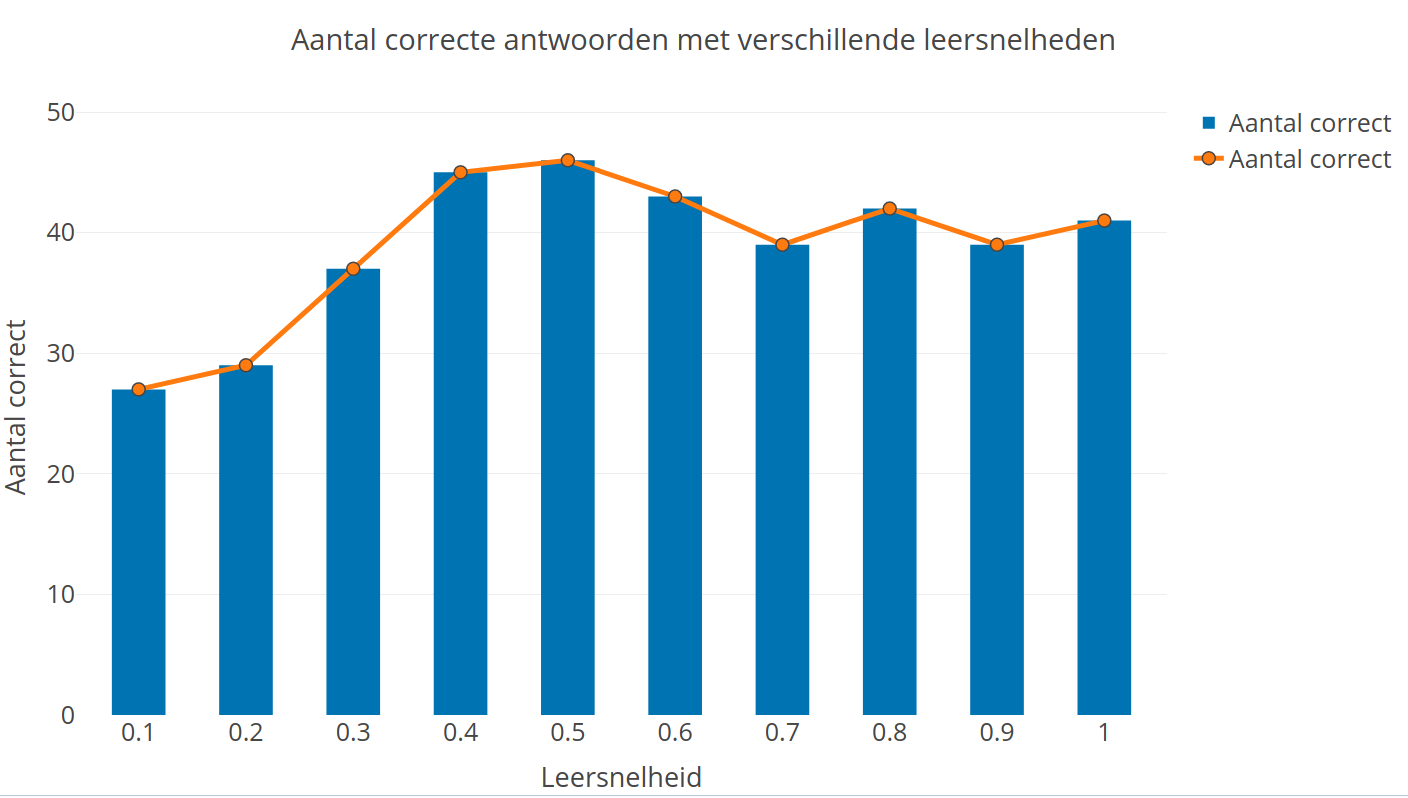
\includegraphics[scale=0.3]{graphs/leersnelheden.png}
    \caption{Aantal correcte antwoorden over 50 executies met verschillende leersnelheden}
    \label{fig:leersneheden}
\end{figure}

We zien in Figuur \ref{fig:leersneheden} dat er wel degelijk een piek is rond een $\alpha$ van 0.5 en dat hogere leersnelheden een lagere hoeveelheid correcte antwoorden geeft. Dit komt, zoals eerder gezegd, doordat hogere leersnelheden ervoor zorgen dat het netwerk zich meer aanpast aan exceptionele gevallen. Een $\alpha$ van 0.5 is groot genoeg dat het netwerk zich voldoende aanpast om zoveel mogelijk het correcte antwoord te geven en klein genoeg dat het exceptionele gevallen niet als de norm gaat zien.
\subsection{Aantal verborgen knopen}
Het aantal verborgen knopen kan voor veel variatie in de antwoorden zorgen. Hoe meer verborgen knopen zich in het netwerk bevinden, hoe meer gewichten het netwerk heeft om bij te stellen. Dit leidt tot antwoorden die meer nauwkeurig zijn.

\begin{table}[ht]
    \centering
      $\begin{array}{c||c|c |}
        \text{Aantal verborgen knopen} & \text{Aantal correct} & \text{Percentage \% correct} \\ \hline
        1 & 0 & 0 \\ \hline
        4 & 19 & 38 \\ \hline
        7 & 30 & 60 \\ \hline
        10 & 29 & 58 \\ \hline
        13 & 35 & 70 \\ \hline
        16 & 42 & 84 \\ \hline
        19 & 43 & 86 \\ \hline
        22 & 43 & 86 \\ \hline
        25 & 42 & 84 \\ \hline
      \end{array}$
    \caption{Aantal correcte antwoorden over 50 executies met verschillende aantallen verborgen knopen}
    \label{tab:hidden}
\end{table}

\begin{figure}[ht]
    \centering
    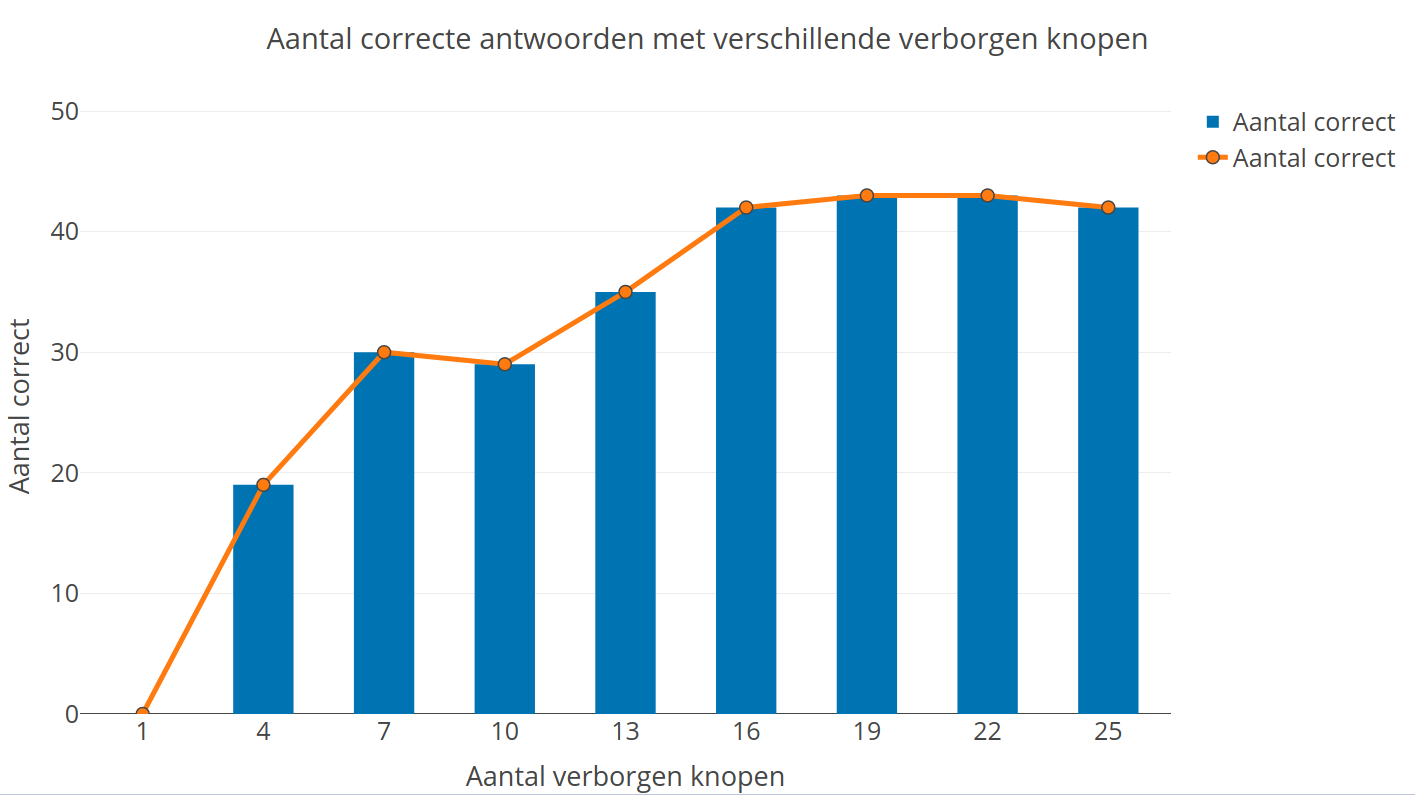
\includegraphics[scale=0.3]{graphs/knopen.png}
    \caption{Grafiek van Tabel \ref{tab:hidden}}
    \label{fig:hidden}
\end{figure}

\subsection{Aantal trainingssessies}
Intu\"itie zegt dat hoe meer gelegenheden het netwerk krijgt om te trainen, hoe beter het netwerk wordt. Hier willen we kijken wat de bovengrens is en tot waar extra trainingssessies weinig invloed hebben op het netwerk.

\begin{table}[ht]
    \centering
      $\begin{array}{c||c|c |}
        \text{Aantal trainingssessies} & \text{Aantal correct} & \text{Percentage \% correct} \\ \hline
        1 & 0 & 0 \\ \hline
        100000 & 15 & 30 \\ \hline
        200000 & 36 & 72 \\ \hline
        300000 & 38 & 76 \\ \hline
        400000 & 44 & 88 \\ \hline
        500000 & 41 & 82 \\ \hline
        600000 & 42 & 84 \\ \hline
        700000 & 43 & 86 \\ \hline
        800000& 46 & 92 \\ \hline
        900000 & 45 & 90 \\ \hline
        1000000 & 43 & 86 \\ \hline
        1100000 & 48 & 96 \\ \hline
        1200000 & 46 & 92 \\ \hline
        1300000 & 48 & 96 \\ \hline
        1400000 & 46 & 92 \\ \hline
        1500000 & 46 & 92 \\ \hline
      \end{array}$
    \caption{Aantal correcte antwoorden over 50 executies met verschillende aantallen trainingssessies}
    \label{tab:training}
\end{table}

\begin{figure}[ht!]
    \centering
    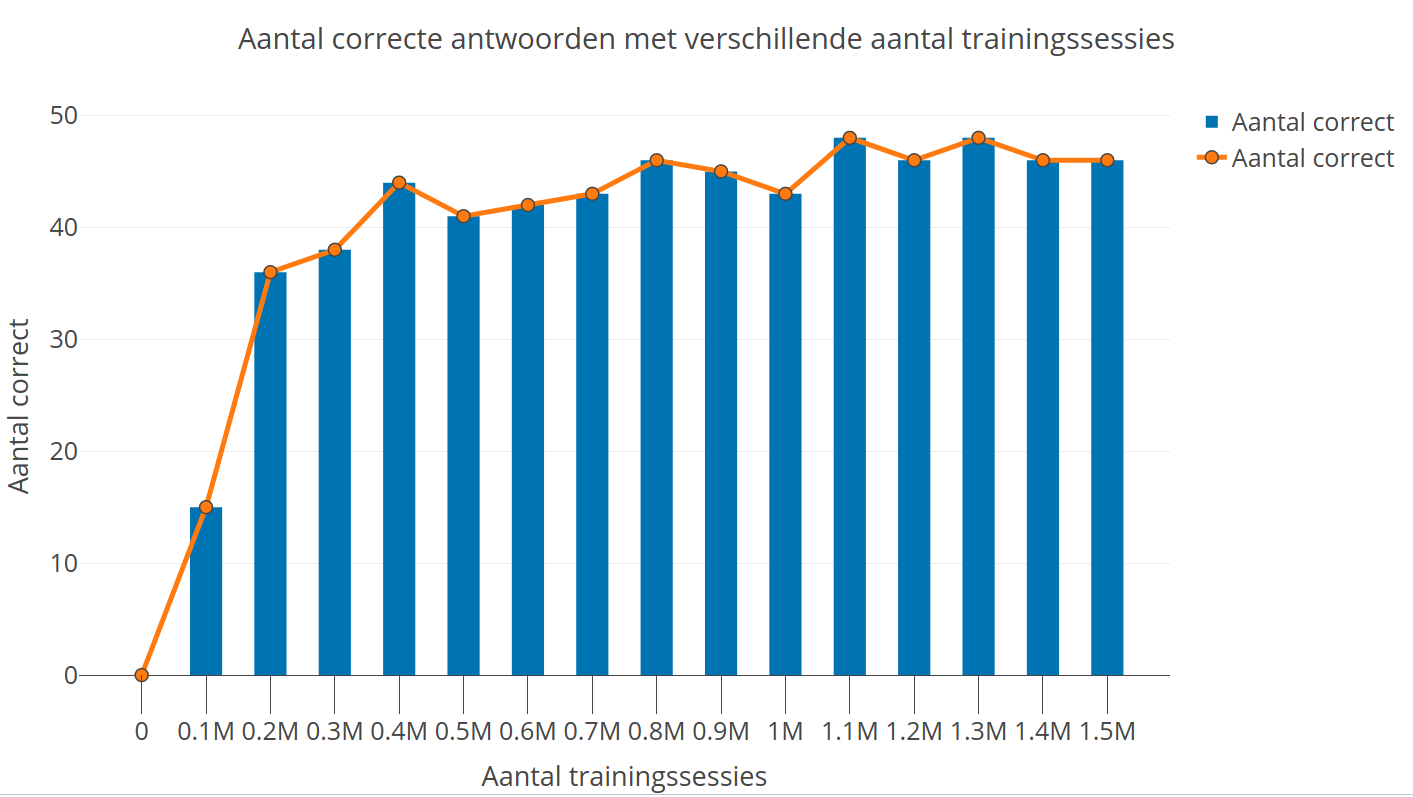
\includegraphics[scale=0.3]{graphs/training.png}
    \caption{Aantal correcte antwoorden over 50 executies met verschillende aantallen trainingssessies}
    \label{fig:training}
\end{figure}

We zien in Tabel \ref{tab:training} en Figuur \ref{fig:training} dat het netwerk inderdaad beter wordt met meer trainingssessies, zoals verwacht. De piek lijkt te zijn geraakt rond de 800000 trainingssessies, waarna er kleine verschillen zijn in opeenvolgende getallen. We kunnen zien dat er wel degelijk een limiet zit aan het aantal trainingssessies dat het netwerk kan doen, voordat het geen effect meer heeft.

\subsection{Aantal inputs}
Het aantal inputs heeft vooral invloed op de ratio van enen en nullen als antwoord. In dit experiment kijken we of het neurale netwerk verschillende hoeveelheden inputs correct kan beantwoorden en of het netwerk sneller leert van meer inputs.

\begin{table}[ht]
    \centering
      $\begin{array}{c||c|c |}
        \text{Aantal inputs} & \text{Aantal correct} & \text{Percentage \% correct} \\ \hline
        2 & 20 & 40 \\ \hline
        4 & 18 & 36 \\ \hline
        6 & 32 & 64 \\ \hline
        0 & 48 & 96 \\ \hline
        10 & 50 & 100 \\ \hline
        12 & 50 & 100 \\ \hline
        14 & 50 & 100 \\ \hline
      \end{array}$
    \caption{Aantal correcte antwoorden over 50 executies met verschillende aantallen inputs}
    \label{tab:inputs}
\end{table}

\begin{figure}[ht!]
    \centering
    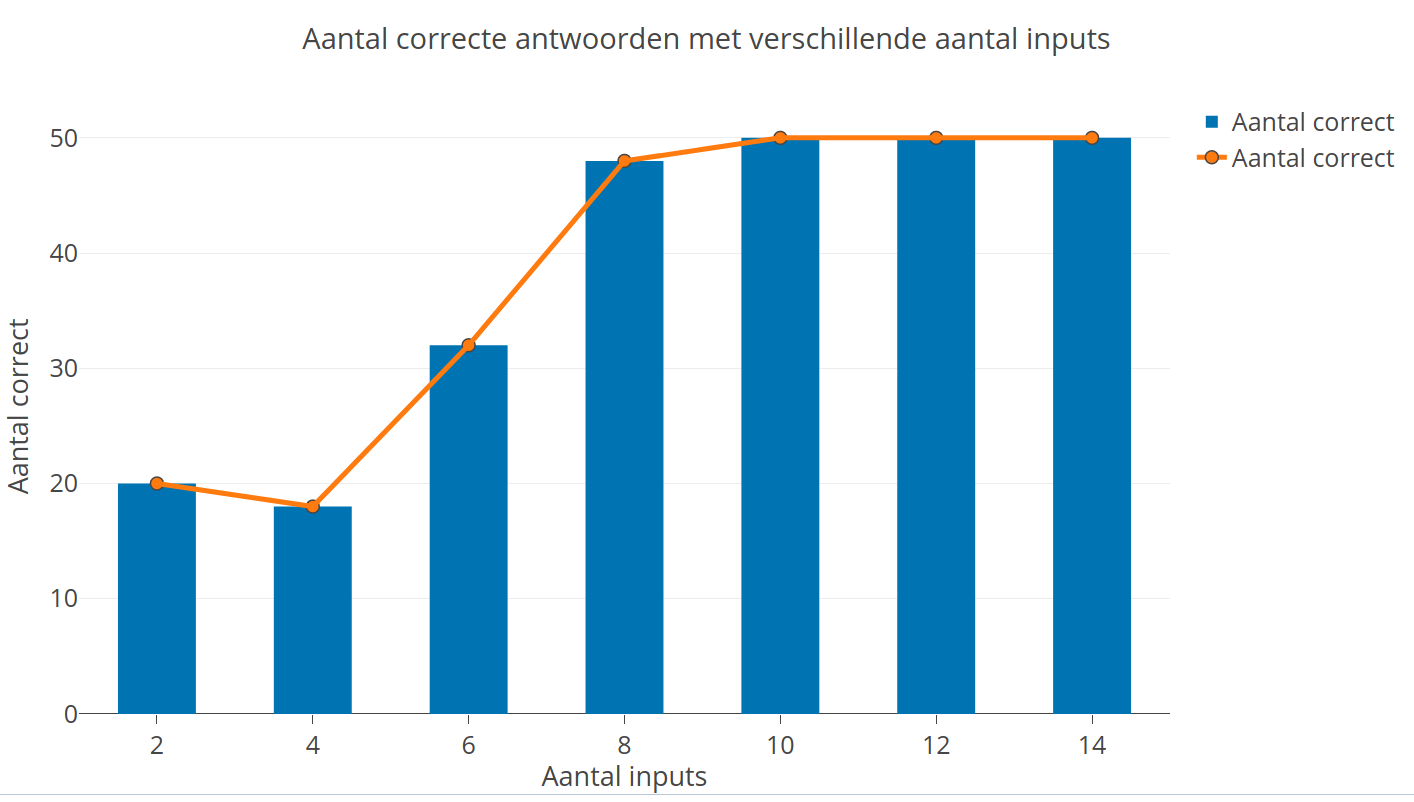
\includegraphics[scale=0.3]{graphs/inputs.png}
    \caption{Aantal correcte antwoorden over 50 executies met verschillende aantallen inputs}
    \label{fig:inputs}
\end{figure}

Meer inputs zorgt ervoor dat het netwerk vaker het correcte antwoord geeft, zoals te zien in Figuur \ref{fig:inputs}. Dit komt doordat de kans dat een XOR operatie 1 teruggeeft exponentieel kleiner wordt als het aantal inputs toeneemt. Voor 2 inputs is er 0.5 kans dat het antwoord een 1 of 0 is. Voor 4 inputs wordt dat $\frac{4}{2^4}$ en $\frac{2^4-4}{2^4}$ kans dat het antwoord een 1 of 0 is respectievelijk. Over het algemeen voor $n$ inputs is de kans dat het antwoord 1 is: $\frac{n}{2^n}$ en de kans dat het antwoord 0 is: $\frac{2^n-n}{2^n}$ of $1-\frac{n}{2^n}$ . Voor grotere $n$ wordt dit:

\begin{align*}
     \text{Het aantal enen: } \lim_{n\to\infty} \frac{n}{2^n} & \approx 0  \\
     \text{Het aantal nullen: } \lim_{n\to\infty} 1 - \frac{n}{2^n} & \approx 1
\end{align*}

Zoals we zien , hoe groter $n$ wordt hoe kleiner de kans dat 1 het antwoord is en hoe groter de kans dat 0 het antwoord is. Dit verklaart het grote success percentage bij grotere inputs. Het netwerk wordt getraind om telkens het antwoord 0 te geven en dit werkt omdat het in de meeste gevallen ook zo is. Het probleem hiervan is dat als een 1 het antwoord is, dat het netwerk dit heel slecht kan beantwoorden en dus vrijwel altijd fout heeft.
\subsection{XOR en OR}
De verschillen tussen het leren van de XOR en OR operaties worden hier onderzocht. Het enige verschil tussen de twee operaties is dat XOR gemiddeld 0.5 kans heeft dat het antwoord 1 of 0 is. OR heeft gemiddeld 0.75 kans dat het antwoord een 1 is en 0.25 kans dat het 0 is.

\begin{table}[ht]
    \centering
      $\begin{array}{l || c | c | c | c}
                                    & \text{Aantal verborgen knopen} & \text{XOR} & \text{OR} \\ \hline
        \text{Aantal correct}       & \multirow{2}{*}{4}  & 26 & 47 \\ \cline{1-1} \cline{3-4}
        \text{Percentage \% correct} &                    & 52 & 94 \\ \cline{1-1} \cline{3-4} \hline \hline
        \text{Aantal correct}       & \multirow{2}{*}{8} & 31 & 50 \\ \cline{1-1} \cline{3-4}
        \text{Percentage \% correct} &                    & 62 & 100 \\ \cline{1-1} \cline{3-4} \hline
      \end{array}$
    \caption{Aantal correcte antwoorden over 50 executies met operaties XOR en OR met verschillende aantallen verborgen knopen}
    \label{tab:xoror}
\end{table}

\begin{figure}[ht!]
    \centering
    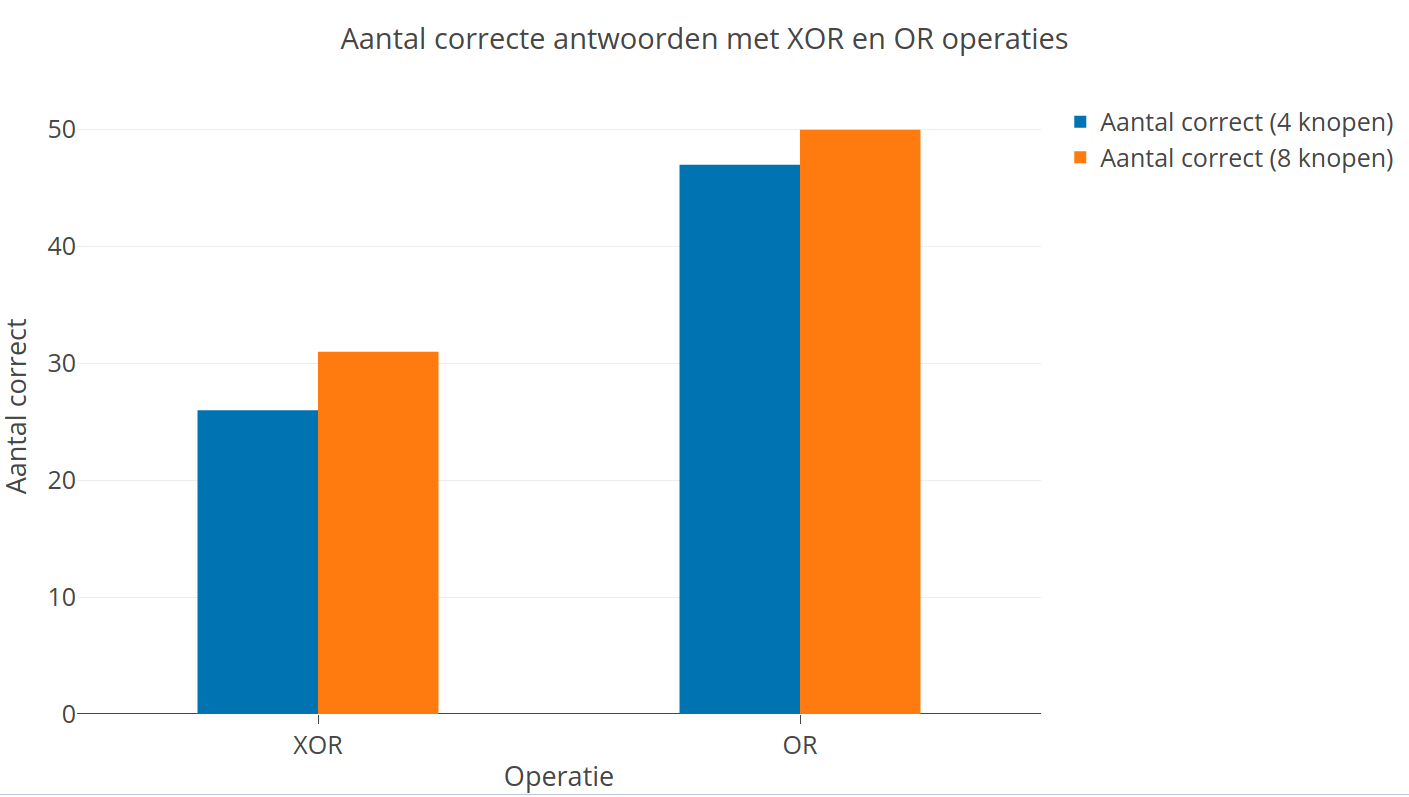
\includegraphics[scale=0.3]{graphs/xoror.png}
    \caption{Grafiek van Tabel \ref{tab:xoror}}
    \label{fig:xoror}
\end{figure}

\subsection{Sigmoid en ReLU}
In dit experiment bekijken we het verschil tussen de activatie functies, sigmoid en ReLU. Het verschil tussen de twee is dat sigmoid een bovengrens van 1 heeft, terwijl ReLU geen boven grens heeft.

\begin{table}[ht]
    \centering
      $\begin{array}{ c || l | c  | c | c}
   \text{Aantal verborgen knopen} & & \text{Sigmoid} & \text{ReLU} \\ \hline
     \multirow{2}{*}{4}  &    \text{Aantal correct}       & 23 & 30 \\ \cline{2-4}
     &   \text{Percentage \% correct} & 46 & 60 \\ \cline{2-4}
     &   \text{Tijd (in secondes)}   & 8.881 & 1.412 \\ \hline \hline 
     \multirow{2}{*}{16} &   \text{Aantal correct}       & 36 & 30 \\ \cline{2-4}
     &   \text{Percentage \% correct} & 72 & 60 \\ \cline{2-4}
     &   \text{Tijd (in secondes)} & 26.516 & 4.219\\ \hline \hline
      \multirow{2}{*}{24} &   \text{Aantal correct}       & 41 & 31\\ \cline{2-4}
     &   \text{Percentage \% correct} & 82 & 62\\ \cline{2-4}
     &   \text{Tijd (in secondes)}  & 38.275 & 6.166\\ \hline
      \end{array}$
    \caption{Aantal correcte antwoorden over 50 executies met activatie functies sigmoid en ReLU met verschillende aantallen verborgen knopen}
    \label{tab:relu}
\end{table}
\begin{figure}[ht!]
    \centering
    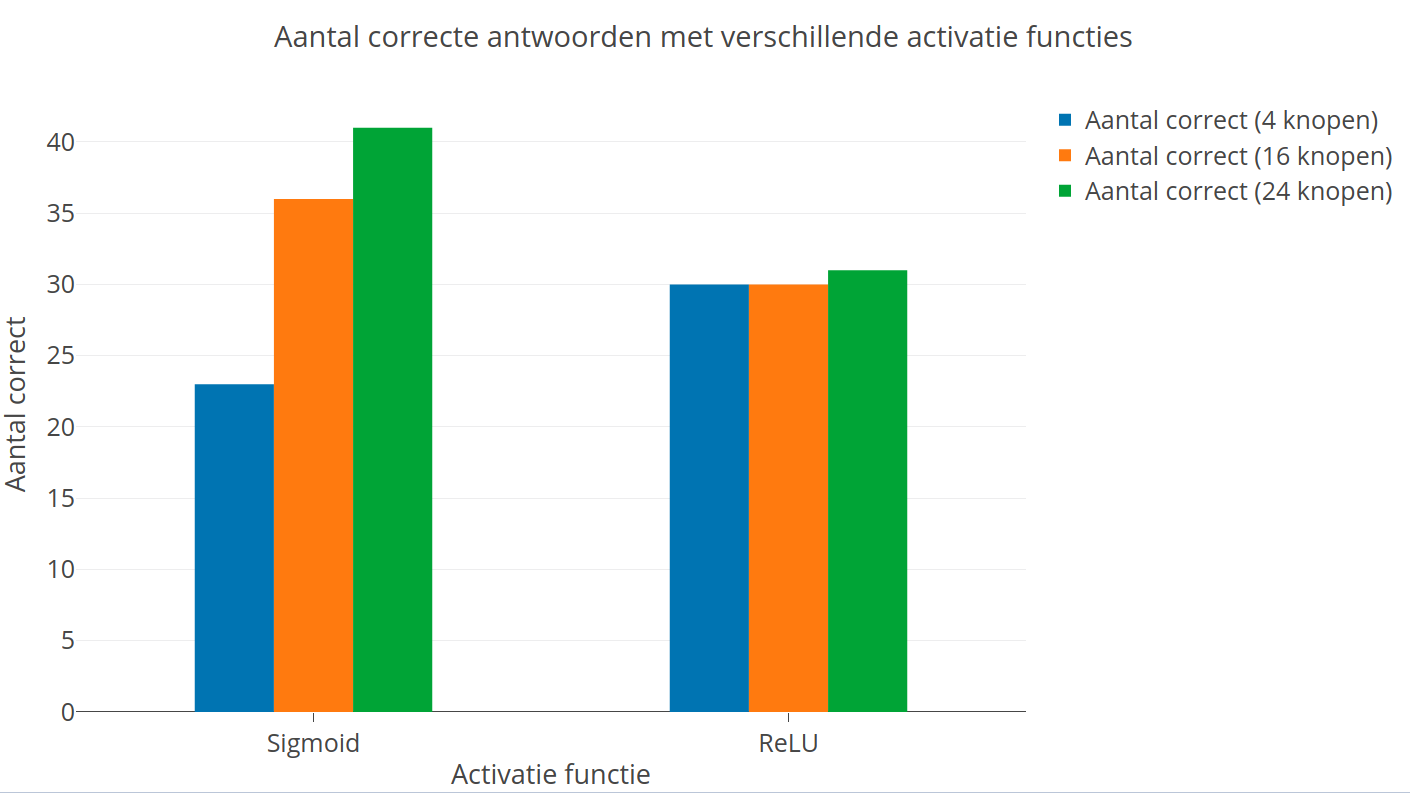
\includegraphics[scale=0.3]{graphs/g.png}
    \caption{Aantal correcte antwoorden over 50 executies met activatie functies sigmoid en ReLU met verschillende aantallen verborgen knopen}
    \label{fig:relu}
\end{figure}

\clearpage
\begin{figure}[ht!]
    \centering
    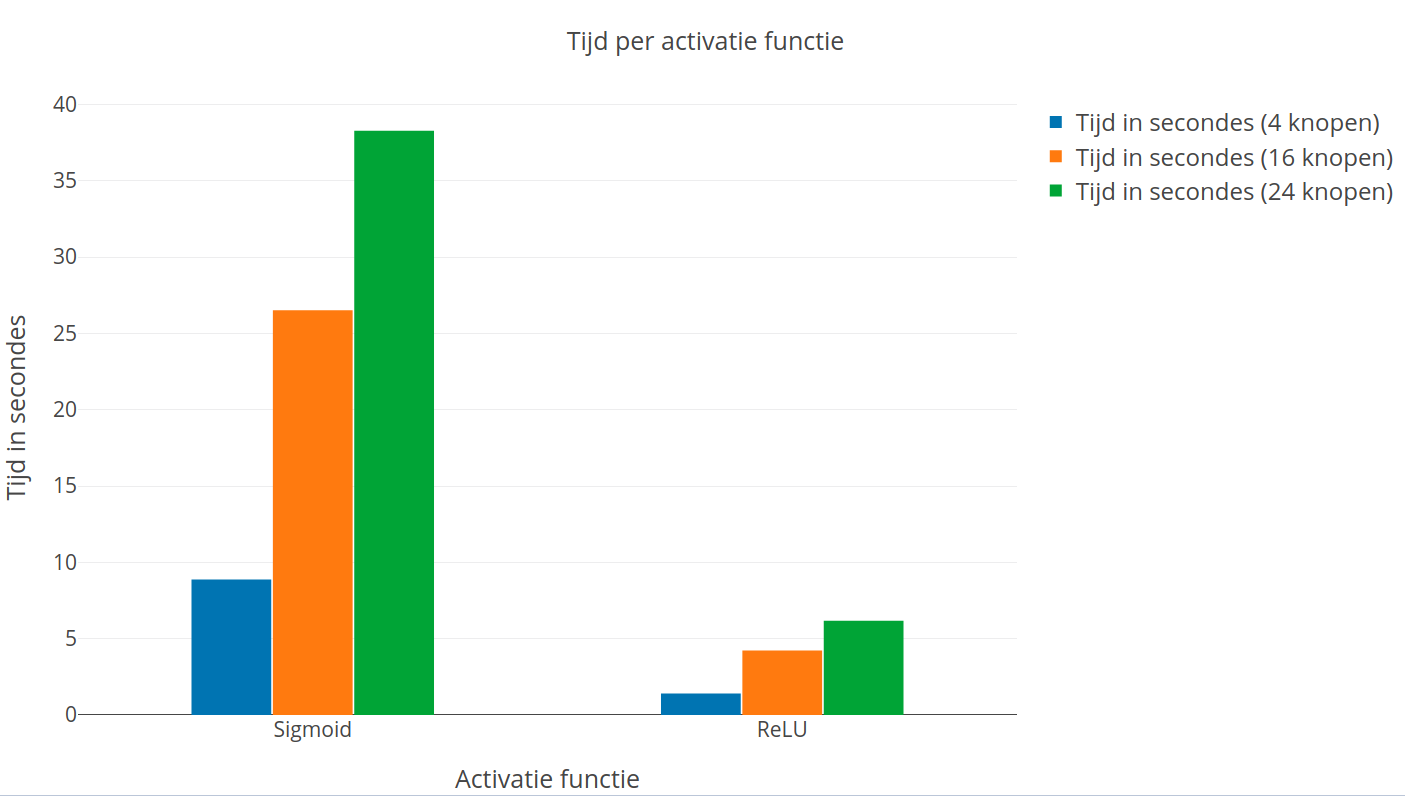
\includegraphics[scale=0.3]{graphs/time.png}
    \caption{Tijd in secondes over 50 executies met activatie functies sigmoid en ReLU met verschillende aantallen verborgen knopen}
    \label{fig:relutime}
\end{figure}

Tabel \ref{tab:relu} en Figuur \ref{fig:relu} laten het aantal correcte antwoorden van het netwerk zien met de activatie functies sigmoid en ReLU voor verschillend aantal verborgen knopen. We zien dat voor een klein aantal verborgen knopen, het netwerk beter leert met ReLU dan met sigmoid. Echter, bij grotere hoeveelheden knopen wordt dit omgedraaid en doet sigmoid het beter dan ReLU. Dit kan komen doordat ReLU geen bovengrens heeft en dus de output van het netwerk groter kan zijn dan 1. We zien wel dat ReLu significant sneller is dan sigmoid en dat de stijging veel sneller is bij sigmoid, zoals te zien op Figuur \ref{fig:relutime}.
Dit is een van de redenen waarom ReLU vaker wordt gebruikt in de praktijk, vooral bij diepere netwerken met meerdere verborgen lagen. Omdat het netwerk daar meer lagen heeft verwachten we dat ReLU beter presteert dan sigmoid in zowel tijd als correctheid. Dit kan worden onderzocht in een volgend onderzoek.
\subsection{Keras netwerk}
Als laatste vergelijken we ons neuraal netwerk met een netwerk gemaakt met behulp van Keras \cite{keras}, een neuraal netwerk API. Het Keras netwerk dat is gebruikt, is te vinden op de opdracht pagina \cite{assignment}. 
Beiden netwerken zullen draaien met 10000 trainingssessies, 2 verborgen knopen met sigmoid als activatie functie en een leersnelheid van 0.01.

\begin{table}[ht]
    \centering
      $\begin{array}{l || c | c | c}
                                     & \text{Keras} & \text{Wij} \\ \hline
        \text{Percentage \% correct} & 51 & 0 \\ \hline
        \text{Tijd}      & 0m10.557s & 0m0.024s \\ \hline
      \end{array}$
    \caption{Het Keras netwerk tegen ons neuraal netwerk}
    \label{tab:keras}
\end{table}

Hier draaien beide netwerken met 500000 trainingssessies, 10 verborgen knopen met sigmoid als activatie functie en een leersnelheid van 0.1.

\begin{table}[ht]
    \centering
      $\begin{array}{l || c |  c | c}
                                     & \text{Keras} & \text{Wij} \\ \hline
        \text{Percentage \% correct} & 100 & 100 \\ \hline
        \text{Tijd}      & 6m56.185s & 0m1.798s  \\ \hline
      \end{array}$
    \caption{Het Keras netwerk tegen ons neuraal netwerk}
    \label{tab:keras}
\end{table}

We zien in Tabel \ref{tab:keras} dat Keras het significant beter doet met een relatief klein aantal verborgen knopen en trainingssessies. Het Keras netwerk behaalde een percentage van 51 terwijl ons netwerk een percentage had van 0. Bij grotere aantallen verborgen knopen en trainingssessies zijn de resultaten van beiden netwerken gelijk. Wel is er een behoorlijk verschil in de tijd om \'e\'en antwoord te geven. Ons netwerk produceert een antwoord vele malen sneller dan het Keras netwerk in beide testen. Uiteindelijk is dit een afweging van de nauwkeurigheid met snelheid. 


\section{Conclusie}
We bespreken nu de conclusies van de verschillende experimenten.

\subsection{Verschillende leersnelheden}
Een leersnelheid van 0.5 laat het neurale netwerk snel genoeg leren om een hoog aantal correcte antwoorden te geven. 

\subsection{Aantal verborgen knopen}
Een hoger aantal knopen leidt inderdaad tot een hoger aantal correcte antwoorden. Deze stijging piekt rond de 22 knopen.

\subsection{Aantal trainingssessies}
Net zoals bij de verborgen knopen, leidt een hoger aantal rainingssessies tot een hoger aantal correcte antwoorden. Er is een punt waar deze stijging piekt en daarna relatief gelijk blijft. Dit is rond de 800000 trainingssessies.

\subsection{Aantal inputs}
Het aantal inputs heeft grote gevolgen voor het leerpatroon van het netwerk. Grotere hoeveelheden inputs verkleinen de kans dat 1 het antwoord is met de XOR operatie, waardoor het netwerk de neiging heeft om alleen maar getallen te produceren die dicht bij 0 zijn. Een exceptie komt voor als 1 het antwoord moet zijn, wat het netwerk bijna nooit goed kan beantwoorden.

\subsection{XOR en OR}
De OR operatie is makkelijker te leren voor het netwerk dan XOR. Dit komt doordat OR een grotere kans heeft om 1 als antwoord te hebben dan XOR. Hierdoor heeft het netwerk de neiging om 1 als antwoord te produceren bij OR en in de meeste gevallen is dit correct. XOR zorgt voor meer variatie en dus meer kans op foute antwoorden.

\subsection{Sigmoid en ReLU}
Sigmoid werkt beter in de meeste gevallen en produceert een stijging in correcte antwoorden bij grotere hoeveelheden knopen. ReLU daarentegen blijft relatief gelijk bij grotere hoeveelheden knopen en produceert minder correcte antwoorden, maar is vele malen sneller dan sigmoid.

\subsection{Keras netwerk}
Het Keras netwerk is aan de hand van de testen veel beter in het produceren van goede antwoorden bij kleinere aantallen verborgen knopen en trainingssessies, terwijl ons netwerk het zeer slecht in zulke gevallen doet. Op grotere hoeveelheden is het gelijk in het produceren van correcte antwoorden. Wel is het Keras netwerk velen malen langzamer dan ons netwerk.

\clearpage

\begin{thebibliography}{XX}

\bibitem{assignment}
W.A. Kosters, \href{http://liacs.leidenuniv.nl/~kosterswa/AI/nn18.html}{\underline{http://liacs.leidenuniv.nl/\textasciitilde{}kosterswa/AI/nn18.html}}, 19 april 2018

\bibitem{keras} 
Keras: The Python Deep Learning library. Bezocht op 15 mei 2018, \href{https://keras.io/}{\underline{https://keras.io/}}

\bibitem{book}
Russell S. \& Norvig P. et al (2009) Artificial Intelligence A Modern Approach Third Edition. New Jersey, NJ, Pearson

\bibitem{chapter}
Russell S. \& Norvig P. et al (2009) Artificial Neural Networks. In Artificial Intelligence A Modern Approach Third Edition (pp. 727-737). New Jersey, NJ, Pearson

\bibitem{backprop}
W.A Kosters, \href{http://liacs.leidenuniv.nl/\textasciitilde{}kosterswa/AI/nnhelp.pdf}{\underline{http://liacs.leidenuniv.nl/\textasciitilde{}kosterswa/AI/nnhelp.pdf}}, 19 april 2018

\bibitem{image}
Artificial neural network [An example artificial neural network with a hidden layer]. (27 december 2006).
Bezocht op 7 mei 2018, 
\href{https://en.wikipedia.org/wiki/Artificial_neural_network#/media/File:Colored_neural_network.svg}{\underline{https://en.wikipedia.org/wiki/Artificial\_neural\_network\#/media/File:Colored\_neural\_network.svg}}

\bibitem{relu} Rectified (neural networks) (20 april 2018) Bezocht op 14 mei 2018, \href{https://en.wikipedia.org/wiki/Rectifier_(neural_networks)}{\underline{https://en.wikipedia.org/wiki/Rectifier\_(neural\_networks)}}


\end{thebibliography}

\clearpage

\section*{Appendix: Code}
Dit is de code voor het neurale netwerk.
\lstinputlisting{nnskelet.cc}

\end{document}